\documentclass[11pt,a4paper]{article}
\usepackage[utf8]{inputenc}
\usepackage[T1]{fontenc}
\usepackage[polish]{babel}
\usepackage{lmodern}
\usepackage{graphicx}
\usepackage{epstopdf}
\usepackage{anysize}
\usepackage{makeidx}
\usepackage{hyperref}
\usepackage{listings}



\makeatletter
\renewcommand{\maketitle}{
\begin{titlepage}
\begin{center}

\LARGE{AKADEMIA GÓRNICZO-HUTNICZA}

\vspace*{1cm}

\includegraphics[scale=1.8]{agh.eps}
\vspace*{1cm}

\LARGE{im. Stanisława Staszica w Krakowie}

\rule{\textwidth}{0.4mm}
\LARGE \textsc{\@title}
\rule{\textwidth}{0.4mm}

\vspace*{5mm}


\large
\emph{Autorzy:}\\
Tomasz \textsc{Czarnik}\\
Krzysztof \textsc{Garcarz}\\
Krzysztof \textsc{Śmiłek}\\

\vfill
\vspace*{\stretch{8}}
\rule{\textwidth}{0.4mm}

\large{Wydział Elektroniki, Automatyki, Informatyki i Elektrotechniki}\\
\large{Katedra Automatyki}\\
\large{Laboratorium Biocybernetyki}\\
\vspace*{\stretch{7}}
\@date

\end{center}

\end{titlepage}
}
\makeatother

\title{Projekt sieci LAN dla szkoły średniej}
\date{\today}

\makeindex

\begin{document}

\maketitle

\newpage

\tableofcontents

\newpage

\section{Wstęp}
\subsection{Cel projektu}
Naszym celem jest stworzenie projektu sieci LAN na potrzeby szkoły średniej przy pomocy technologii poznanych na zajęciach z przedmiotu Administrowanie sieciami lokalnymi. Staraliśmy się użyć, w rozsądnych granicach jak najwięcej poznanych narzędzi.
\subsection{Założenia projektu}
Przyjęliśmy następujące założenia odnośnie sieci:
\begin{itemize}
\item Szkoła posiada dwie pracownie komputerowe na parterze i na pierwszym piętrze, każda z nich liczy po 12 komputerów
\item Dodatkowo istnieje potrzeba podłączenia do sieci sekretariatu, gabinetu dyrektora oraz komputera w pokoju nauczycielskim
\item W sieci pracują również dwa serwery
\item Adresy komputerów obu pracowni przydzielane są przez DHCP
\item Sieć będzie działać w topologii rozszerzonej gwiazdy
\end{itemize}
\subsection {Urządzenia i okablowanie}
Przy realizacji naszej sieci skorzystalibyśmy z dwóch routerów oraz paru switchy. Routery zestawione są serialami, natomiast wszystkie pozostałe urządzenia za pomocą portów FastEthernet połączone skrętką (kablem typu UTP kategorii 5).\\
Kablem skrosowanym połączyliśmy urządzenia tego samego typu (Router-Komputer, Switch-Switch) natomiast prostym urządzenia różnego typu (Router-Switch, Switch-Komputer).

\section{Projekt sieci}
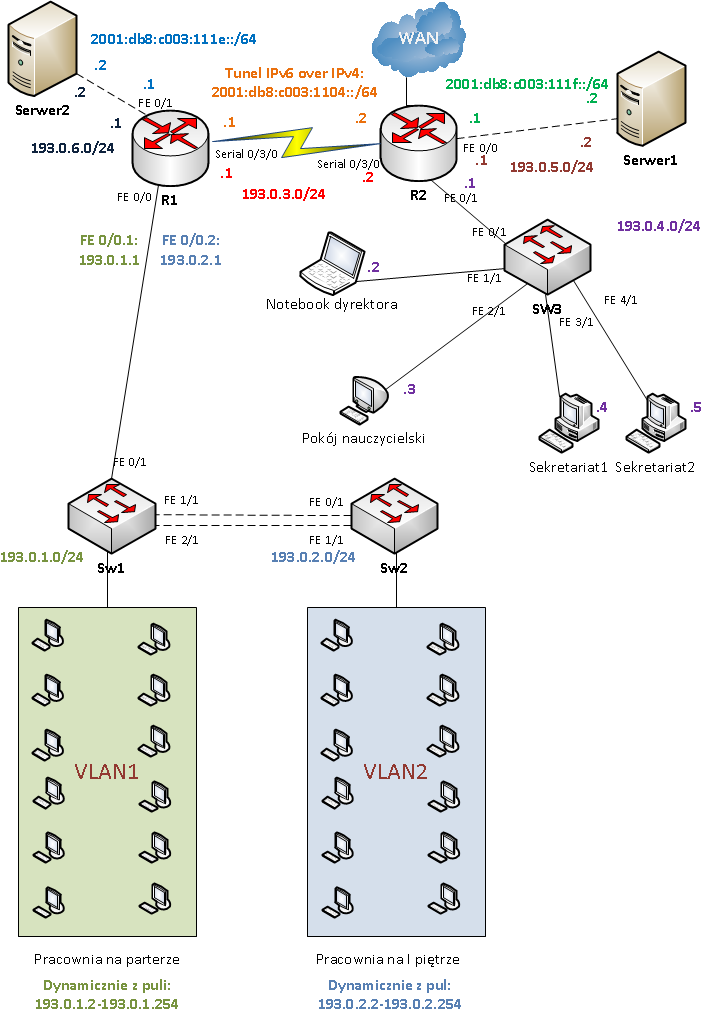
\includegraphics[scale=0.6]{siec.png}  

\section{Konfiguracja}

%===========================================================
\subsection{Konfiguracja interfejsów routerów}
{\bf R1:}\\
\noindent
Ustawienie interfejsów i subinterfejsów FastEthernet:
\begin{lstlisting}
R1(config)#interface fastEthernet 0/0.1
R1(config-subif)#ip address 193.0.1.1 255.255.255.0
R1(config-subif)#no shutdown
R1(config-subif)#encapsulation dot1Q 1

R1(config)#interface fastEthernet 0/0.2
R1(config-subif)#ip address 193.0.2.1 255.255.255.0
R1(config-subif)#no shutdown
R1(config-subif)#encapsulation dot1Q 2

R1(config)#interface fastEthernet 0/1
R1(config-if)#ip address 193.0.6.1 255.255.255.0
R1(config-if)#no shutdown
\end{lstlisting}

\noindent
{\bf R2:}\\
Ustawienie interfejsów FastEthernet:
\begin{lstlisting}
R2(config)#interface fastEthernet 0/0
R2(config-subif)#ip address 193.0.5.1 255.255.255.0
R2(config-subif)#no shutdown

R2(config)#interface fastEthernet 1/0
R2(config-subif)#ip address 193.0.4.1 255.255.255.0
R2(config-subif)#no shutdown
\end{lstlisting}

%===========================================================
\subsection{Konfiguracja switchy}
{\bf Sw1 i Sw2}\\
Stworzenie dodatkowego vlana o numerze 2:
\begin{lstlisting}
Sw1(config)#vlan 2
Sw1(config-vlan)#name VLan2
\end{lstlisting}
\noindent
{\bf Sw1}\\
Stworzenie łącza trunk:
\begin{lstlisting}
Sw1(config)#interface FastEthernet0/1
Sw1(config-if)#switchport mode trunk
Sw1(config-if)# switchport trunk encapsulation dot1q
\end{lstlisting}
Przypisanie portów do danych VLANów (przypisujemy tylko do VLAN 2, bo reszta połączeń jest automatycznie przypisywana do VLAN 1):
\begin{lstlisting}
Sw1(config)#interface FastEthernet1/1
Sw1(config-if)#switchport mode access
Sw1(config-if)#switchport access vlan 2
\end{lstlisting}

\noindent
{\bf Sw2}\\
Przypisanie wszystkich portów do VLan2:
Dla każdego z interfejsów (X-numer interfejsu):
\begin{lstlisting}
Sw2(config)#interface FastEthernet X
Sw2(config-if)#switchport mode access
Sw2(config-if)#switchport access vlan 2
\end{lstlisting}
Powyższe dzialanie sprawia, że protokół STP poprawnie tworzy drzewo rozpinające dla każdego z Vlanów.

%===========================================================
\subsection{Listy ACL}
Listy kontroli dosępu (ACL) mają za zadanie uniemożliwić komunikowanie się pracowni komputerowych z komputerami znajdującymi się w sekretariacie za wyjątkiem polecenia ping. Na routerze R1 tworzona jest access lista:
\begin{lstlisting}
R1# conf t
R1(config)#access-list 101 permit icmp any 193.0.4.0 0.0.0.255 
R1(config)#access-list 101 deny ip 193.0.0.0 0.0.255.255 193.0.4.0 0.0.0.255
R1(config)#access-list 101 permit ip any any
\end{lstlisting}
Następnie aktywujemy access listę na danym porcie:
\begin{lstlisting}
R1(config)# interface Serial 0/3/0
R1(config-if)#ip access-group 101 out	
R1(config-if)#exit 
\end{lstlisting}
Przy takiej konfiguracji powinno się dać z komputerów pracowni jedynie pingować komputer w sekretariacie.

%===========================================================
\subsection{STP}
Aby przetestować protokół STP pomiędzy switchami Sw1 i Sw2 ustanowiliśmy dodatkowe, nadmiarowe połączenie. Chcemy wybrać interfejs, który zostanie przełączony w stan 'Alternate'. W tym celu zwiększamy koszt połączenia z jednego z interfejsów:
\begin{lstlisting}
Sw1>enable
Sw1#conf t
Sw1(config)#interface Ethernet 2/1
Sw1(config-if)#spanning-tree cost 200
Sw1(config-if)#exit
Sw1(config)#exit
\end{lstlisting}

%===========================================================
\subsection{Routing}
{\bf R1:}\\
\begin{lstlisting}
R1(config)#router ospf 1
R1(config-router)#network 193.0.3.0 0.0.0.255 area 1
R1(config-router)#redistribute rip subnets 
 \end{lstlisting}
{\bf R2:}\\
\begin{lstlisting}
R2(config)#router rip
R2(config-router)#version 2
R2(config-router)#passive-interface FastEthernet0/0
R2(config-router)#network 193.0.4.0
R2(config-router)#network 193.0.5.0
R2(config-router)#no auto-summary

R2(config)#router ospf 1
R2(config-router)#network 193.0.3.0 0.0.0.255 area 1
R2(config-router)#redistribute rip subnets 
 \end{lstlisting}
%===========================================================
\subsection{NAT}

Chcemy sprawić, aby komputery z obu pracowni były widziane na zewnątrz pod jednym adresem, w tym celu skonfigurujemy NAT.\\
Najpierw upewniamy się, iż adresy sieciowe obu VLANów są odłączone z routringu i komputery z zewnątrz nie są widoczne.\\
Następnie definiujemy na routerze R1, które interfejsy są wewnętrzne a które prowadzą na zewnątrz:
\begin{lstlisting}
R1(config)#interface FastEthernet 0/0.1
R1(config-subif)#ip nat inside

R1(config)#interface FastEthernet 0/0.2
R1(config-subif)#ip nat inside

R1(config)#interface serial 0/3/0
R1(config-if)#ip nat outside
\end{lstlisting}
Tworzymy access listę opisującą zakres adresów tłumaczonych na granicy i tworzymy translację:
\begin{lstlisting}
R1(config)#access-list 1 permit 193.0.1.0 0.0.0.255
R1(config)#access-list 1 permit 193.0.2.0 0.0.0.255

R1(config)# ip nat inside source list 1 interface Serial 0/3/0 overload
\end{lstlisting}
Od tej pory komputery wewnątrz NAT widziane są na zewnątrz pod wspólnym adresem (outside - czyli 193.0.3.1).\\
Sprawdziliśmy działanie przez poleceniem ping: z pracowni dało się spingować serwer, natomiast serwer nie mógł pingować komputerów znajdujących się za NATem.
 
%===========================================================

\subsection{DHCP}
Router R1 będzie przydzielał adresy IP dla komputerów obu pracowni poprzez DHCP.\\
Najpierw konfigurujemy pule adresów:
\begin{lstlisting}
R1(config)#ip dhcp pool PracowniaParter
R1(dhcp-config)#network 193.0.1.0 255.255.255.0
R1(dhcp-config)#default-router 193.0.1.1

R1(config)#ip dhcp pool PracowniaPietro
R1(dhcp-config)#network 193.0.2.0 255.255.255.0
R1(dhcp-config)#default-router 193.0.2.1
\end{lstlisting}
Następnie wyłączamy adresy przydzielone statycznie (interfejs routera):
\begin{lstlisting}
R1(config)#ip dhcp excluded-address 193.0.1.1
R1(config)#ip dhcp excluded-address 193.0.2.1
\end{lstlisting}

Sprawdzamy działanie DHCP poleceniem show ip dhcp binding:
\begin{lstlisting}
IP address       Client-ID/              Lease expiration        Type
                 Hardware address
193.0.1.2        00E0.B0DE.39E2           --                     Automatic
193.0.1.3        0009.7CB3.E46D           --                     Automatic
193.0.2.3        0003.E460.873B           --                     Automatic
193.0.2.2        00E0.A305.48C0           --                     Automatic
\end{lstlisting}
Jak widać DHCP działa poprawnie dla obu VLANów (oczywiście w rzeczywistości byłoby po 12 komputerów na pracownię).

%===========================================================
\subsection{Most IPv6}

\noindent
Ustawienie mostka IPv6 między routerami {\bf R1 - R2}
\begin{lstlisting}
R1(config)# ???
R1(config-if)# ???
R1(config-if)#???
\end{lstlisting}

\begin{lstlisting}
R2(config)# ???
R2(config-if)# ???
\end{lstlisting}

\section{Podsumowanie}
Przetestowaliśmy wyżej wymienioną konfigurację za pomocą programu Cisco Packet Tracer dla wszystkich sieci działających w IPv4. Niestety program nie radzi sobie z tunelowaniem IPv6 over IPv4, dlatego też nie jesteśmy pewni czy udało nam się odtworzyć sukces z zajęć. 

\end{document}
